\documentclass[10pt,a4paper]{article}
\usepackage[utf8]{inputenc}
\usepackage[italian]{babel}
\usepackage{amsmath}
\usepackage{amsfonts}
\usepackage{amssymb}
\usepackage{graphicx}
\usepackage{siunitx}
\usepackage[left=2cm,right=2cm,top=2cm,bottom=2cm]{geometry}
\newcommand{\rem}[1]{[\emph{#1}]}
\newcommand{\exn}{\phantom{xxx}}
\usepackage[italian]{babel}
\usepackage[utf8]{inputenc}
\usepackage{siunitx}
\usepackage{graphicx}
\usepackage{xcolor}
\usepackage{amsfonts}
\usepackage{amsmath}
\usepackage{amsthm}
\usepackage{tikz}
\usepackage{pgfplots}
\usepackage{enumitem}
\usepackage{subcaption}
\usepackage{siunitx}
\date{\today}
\usetikzlibrary{shapes.geometric,calc,matrix,arrows,snakes,shapes,patterns}
\title{Esercitazione 12B: Macchine e stati finiti:semaforo}
\author{Massimo Bilancioni, Alessandro Foligno, Giuseppe Zanichelli}
\begin{document}	
\maketitle
Si decide arbitrariamente di assegnare i vari stati di $Q_0$ e $Q_1$ ad altrettante posizioni del semaforo. In particolare, la corrispondenza scelta è:\\
\begin{enumerate}
	\item Lo stato (0,0) corrisponde al Verde
	\item Lo stato (0,1) corrisponde al Giallo+Verde
	\item Lo stato (1,0) corrisponde al Rosso
	\item Lo stato (1,1) corrisponde allo stato non desiderato che non rientra del ciclo (in termini di colori per semplificare la  logica  l'abbiamo fatto corrispondere al Rosso+Giallo)
\end{enumerate}
Utilizzando questa corrispondenza, lo schema della transizione è riportato nella seguente tabella (insieme con i valori corrispondenti dei led)\
\begin{table}[h]\centering
\begin{tabular}{|c|c|c|c|c|c|c|}
	\hline 
	$Q_0^n$ & $Q_1^n$ & $Q_0^{n+1}$ & $Q_1^{n+1}$ & Verde & Giallo & Rosso \\ 
	\hline 
	0 & 0 & 0 & 1 & 1 & 0 & 0 \\ 
	\hline 
	0 & 1 & 1 & 0 & 1 & 1 & 0 \\ 
	\hline 
	1 & 0 & 0 & 0 & 0 & 0 & 1 \\ 
	\hline 
	1 & 1 & x & x & x & x & x \\ 
	\hline 
\end{tabular} 	
\caption{Tabella di transizione per $Q_0$ e $Q_1$}
\end{table}
\\
osservando la tabella si vede che il segnale su Verde è proprio $\overline{Q_0}$ (ponendo $x =0$), quello su Giallo è $Q_1$ (ponendo $x= 1$), quello su Rosso è $Q_0$ (ponendo $x= 1$).\\
Per realizzare le transizioni, imponiamo che sia $Q_0^{n+1}=Q_1^n$ e $Q_1^{n+1}=\bar{Q}_0^n \cdot \bar{Q}_1^n$ (questo fa anche in modo che il valore di $(Q_0,Q_1)=(1,1)$ indesiderato non vada in se stesso.)\\
Si riporta lo schema del circuito realizzato in Figura \ref{fig:circ}:

\begin{figure}[h]

			\centering

			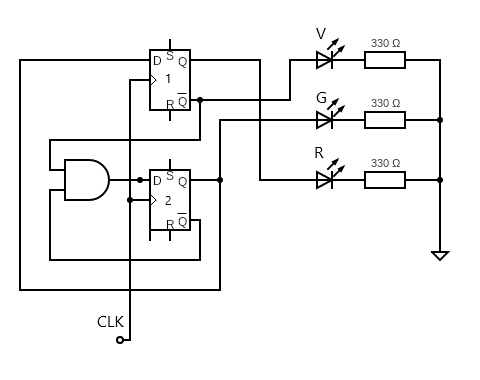
\includegraphics[scale=0.8]{circuit}

			\caption{Implementazione semaforo}

			\label{fig:circ}

\end{figure}


\section{Forme d'onda}
Si monta il circuito illustrato, e si osservano le seguenti forme d'onda sull'oscilloscopio:
\begin{figure}\centering
	\includegraphics[scale=0.7]{green.png}
	\caption{forma d'onda del segnale sul led Verde (arancione), notare come il tempo in cui sta acceso sia il doppio di quello in cui è spento, in blu è riportato il clock}
	
\end{figure}
\begin{figure}
	\includegraphics[scale=0.7]{yellow.png}
	\includegraphics[scale=0.7]{yellowandgreen.png}
	\caption{a sinistra: Segnale (in arancio) sul led Giallo, a destra: segnale sul Verde(arancio) e Giallo(blu): notare che il Giallo si accende solo quando il Verde è già acceso }
	
\end{figure}
\begin{figure}
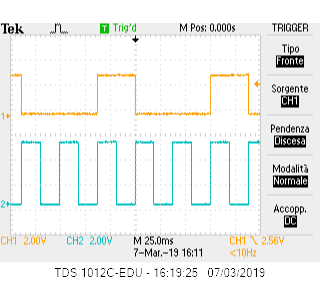
\includegraphics[scale=0.7]{Red.png}
\includegraphics[scale=0.7]{GreenandRed.png}

\end{figure}

\end{document}